\documentclass[11pt]{article}
\usepackage[margin=1in]{geometry}
\usepackage{amsmath}
\usepackage{graphicx}
\usepackage{booktabs}
\usepackage[hidelinks]{hyperref}
\usepackage{parskip}

\title{AI Data Centers and Capacitor Availability:\\
\large Murata's Capacitor Book-to-Bill vs.\ Nvidia Data-Center Revenue, 2024--2026}
\author{Jack R.\ Chepin}
\date{October 2026}

\begin{document}
\maketitle

\section{Motivation}
Multilayer ceramic capacitors (MLCCs) are tiny components that stabilize the power supply to chips.
An AI server board uses thousands of them; industry estimates put AI servers at 10--15 times the
MLCC content of a general-purpose server, and they rely on high-capacitance and high-voltage parts.
This project asks whether the AI data-center buildout has tightened the \emph{availability} of
capacitors, and whether availability tightened before prices responded.

In a supply-constrained market, a demand shock can show up first as longer waits and growing
order backlogs rather than as higher prices, because large buyers purchase on contracts that reset
with a lag. Measuring availability directly is therefore central to the analysis.

\section{Data}
\begin{itemize}
  \item \textbf{Murata Manufacturing}, the largest MLCC producer: quarterly orders received, sales
        shipped and order backlog for the capacitor segment (millions of yen), from Murata's
        quarterly \emph{Consolidated Financial Results} (July 2025 -- July 2026 reports).
        January--March quarters are derived as full-year minus nine-month totals.
  \item \textbf{Nvidia}: quarterly data-center revenue (\$ billions) from Nvidia's quarterly
        results releases. Some quarters are derived from reported growth rates. Nvidia's fiscal
        quarters end about one month after Murata's, so each Murata quarter is paired with the
        Nvidia quarter that mostly overlaps it.
\end{itemize}

\section{Measure of availability}
The outcome is Murata's capacitor \emph{book-to-bill} ratio:
\begin{equation}
  \text{BTB}_t = \frac{\text{Orders}_t}{\text{Sales}_t}.
\end{equation}
A value above 1 means customers are ordering more than the company can ship, so unfilled orders
accumulate and availability tightens.

\begin{table}[h]
\centering
\begin{tabular}{lrrrr}
\toprule
Quarter & Orders (JPY mn) & Sales (JPY mn) & Book-to-bill & Nvidia DC (\$B) \\
\midrule
Apr--Jun 2024 & 213,226 & 203,313 & 1.05 & 26.3 \\
Jul--Sep 2024 & 204,681 & 213,999 & 0.96 & 30.7 \\
Oct--Dec 2024 & 207,210 & 213,089 & 0.97 & 35.6 \\
Jan--Mar 2025 & 207,567 & 201,444 & 1.03 & 39.3 \\
Apr--Jun 2025 & 223,995 & 217,330 & 1.03 & 41.0 \\
Jul--Sep 2025 & 241,807 & 237,572 & 1.02 & 51.1 \\
Oct--Dec 2025 & 268,055 & 239,114 & 1.12 & 62.3 \\
Jan--Mar 2026 & 329,712 & 242,402 & 1.36 & 75.4 \\
Apr--Jun 2026 & 415,505 & 282,508 & 1.47 & 89.0 \\
\bottomrule
\end{tabular}
\caption{Murata capacitor segment and paired Nvidia data-center revenue.}
\end{table}

\section{Method}
I report the Pearson correlation, the Spearman rank correlation, and an ordinary least squares
regression:
\begin{equation}
  \text{BTB}_t = \alpha + \beta\,\text{NvidiaDC}_t + \varepsilon_t ,
\end{equation}
where $\text{NvidiaDC}_t$ is Nvidia's data-center revenue in the overlapping quarter.
The analysis is implemented in base R (\texttt{murata\_vs\_nvidia\_base.R}).

\section{Results}
\begin{table}[h]
\centering
\begin{tabular}{lr}
\toprule
Statistic & Value \\
\midrule
Pearson $r$ & 0.92 \\
Spearman $\rho$ & 0.70 \\
$\hat\beta$ (per \$1B of Nvidia DC revenue) & 0.0078 (s.e.\ 0.0012) \\
$\hat\alpha$ & 0.723 (s.e.\ 0.067) \\
$t$-statistic on $\hat\beta$ & 6.28 \\
$p$-value on $\hat\beta$ & 0.0004 \\
$R^2$ & 0.85 \\
Observations & 9 \\
\bottomrule
\end{tabular}
\caption{Book-to-bill regressed on Nvidia data-center revenue.}
\end{table}

\begin{figure}[h]
\centering
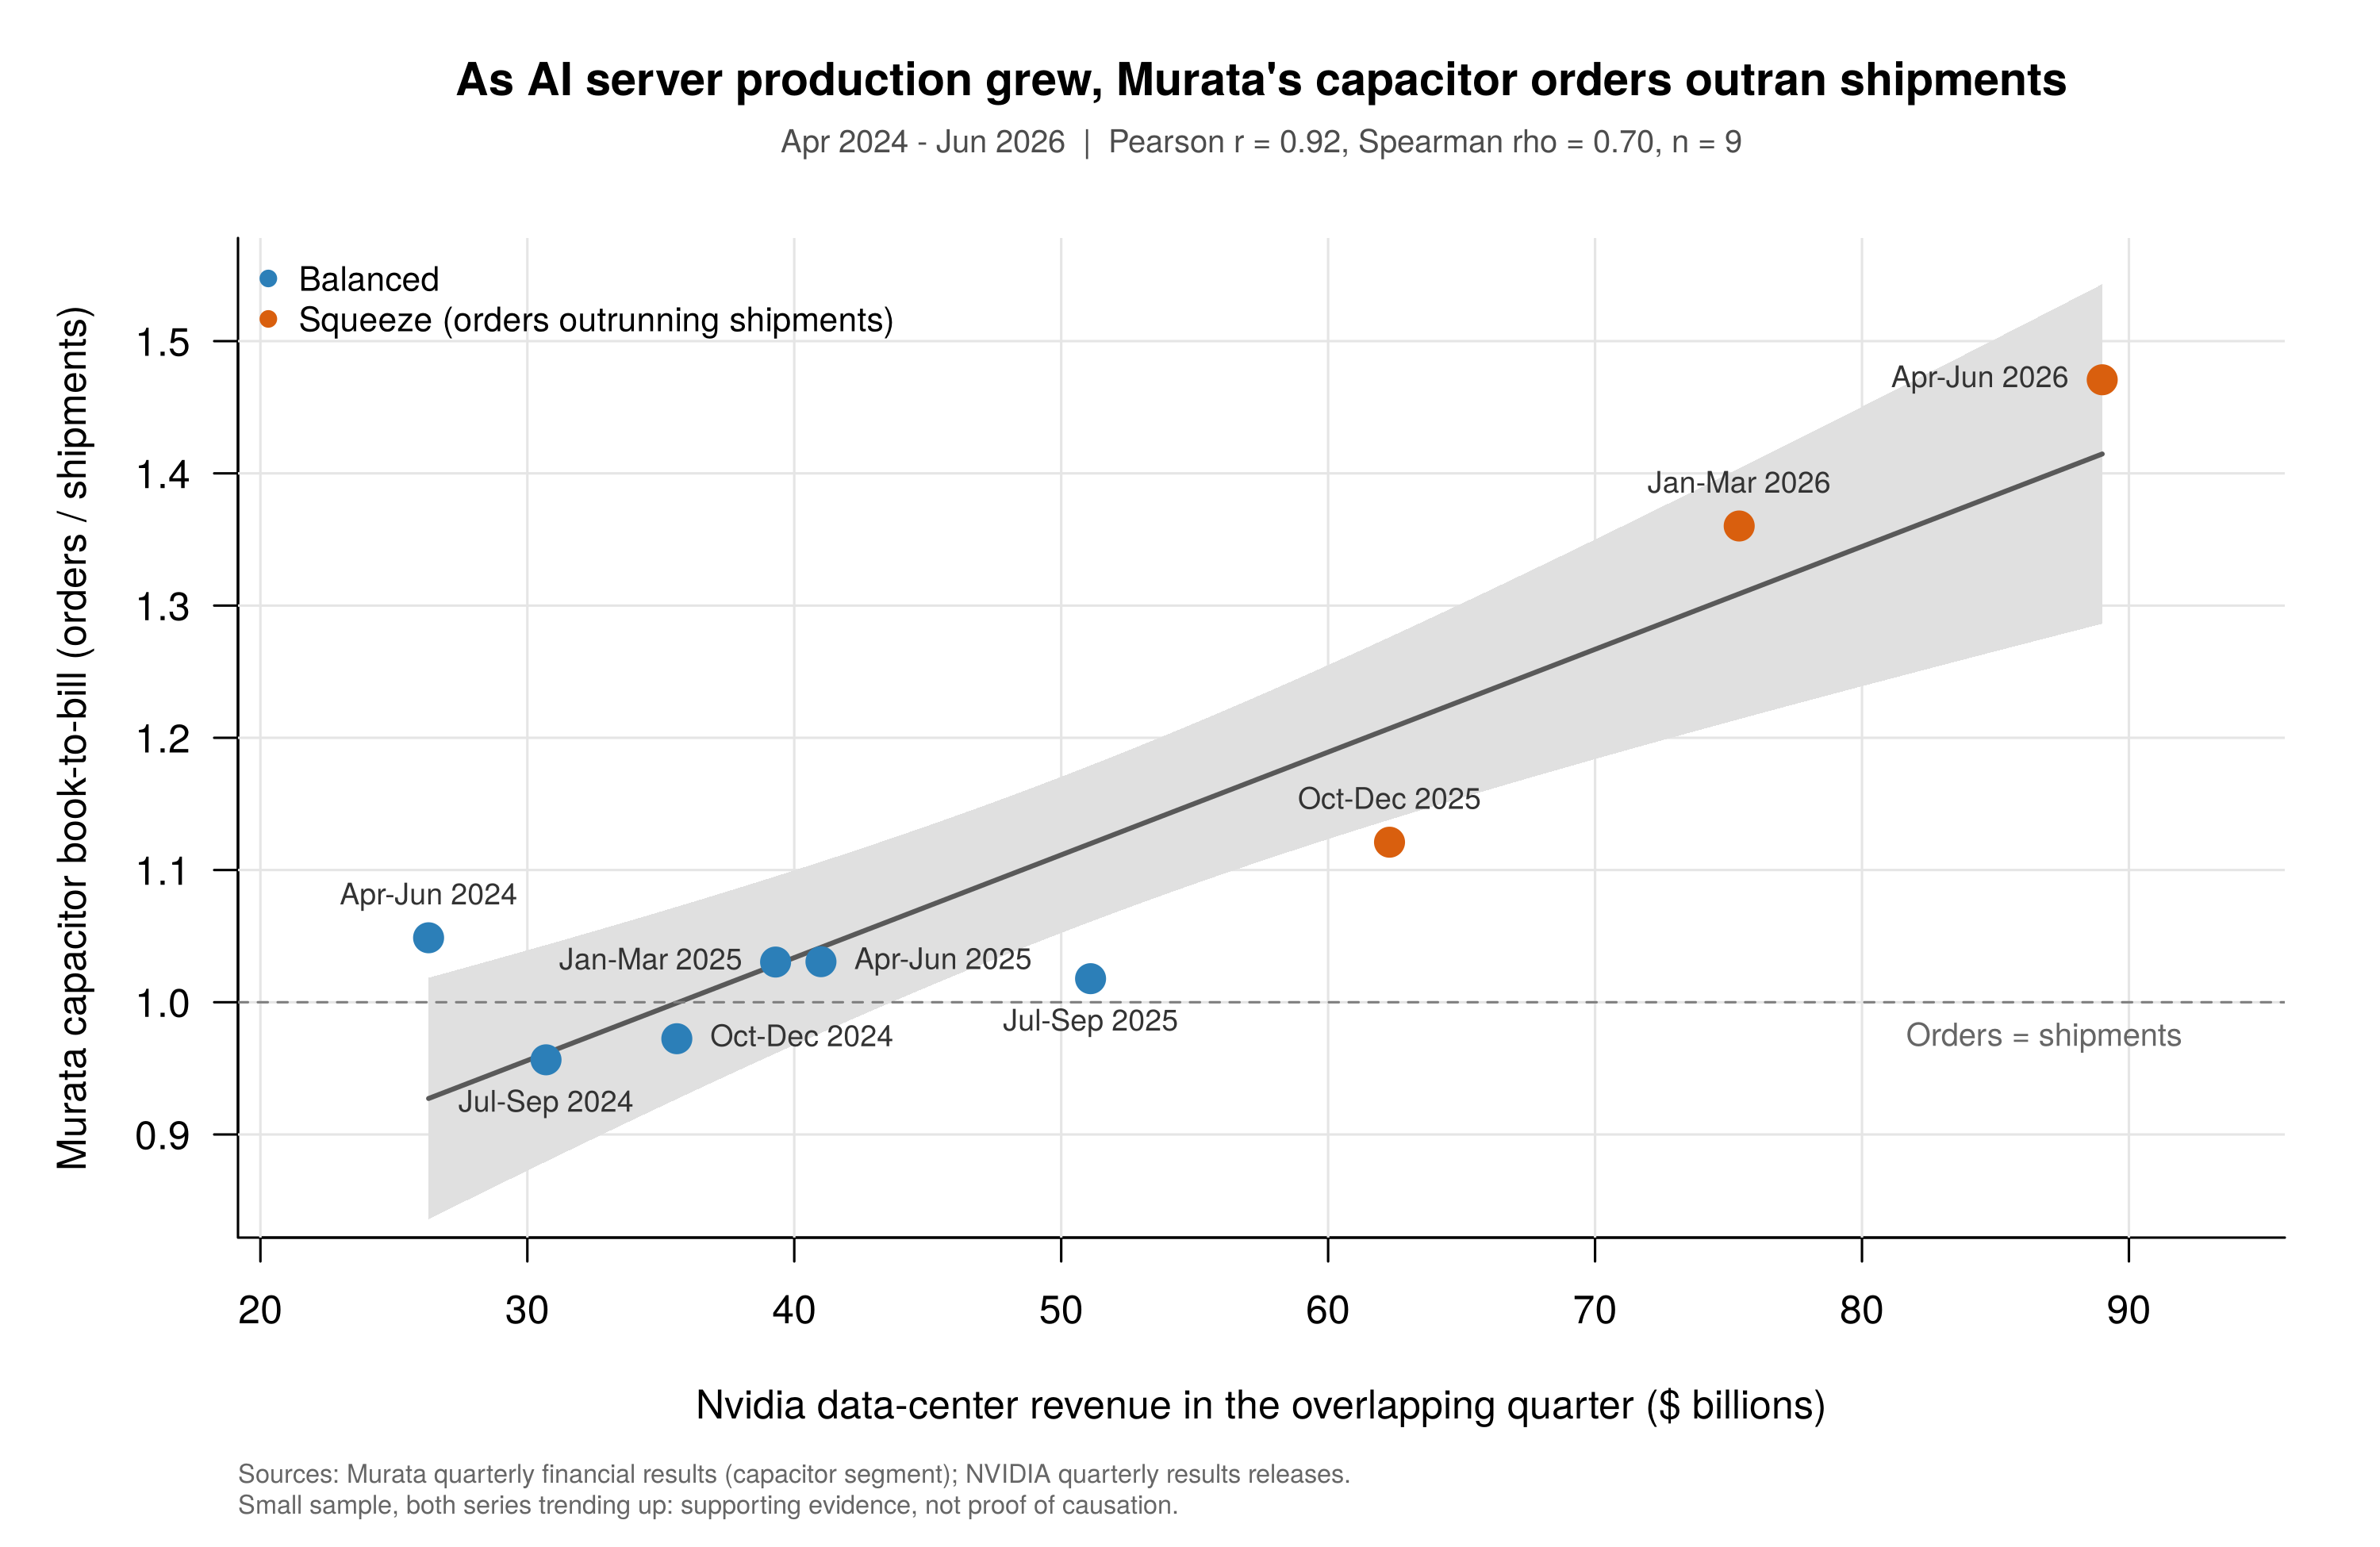
\includegraphics[width=0.85\textwidth]{../murata_vs_nvidia_base.png}
\caption{Murata capacitor book-to-bill vs.\ Nvidia data-center revenue by quarter.}
\end{figure}

Each additional \$10 billion of quarterly Nvidia data-center revenue is associated with roughly a
0.08 increase in Murata's capacitor book-to-bill. Through September 2025, orders and shipments
were balanced (book-to-bill $\approx 1$) as Murata expanded output. Once Nvidia's quarterly
growth re-accelerated in late 2025, orders pulled ahead: book-to-bill rose to 1.12, 1.36 and 1.47
over the next three quarters, and Murata's backlog rose from about 2 to 4.3 months of sales.
The July--September 2025 quarter sits below the fitted line, consistent with a one-quarter lag.

Over the same period Murata reported falling selling prices in every quarter through June 2026,
and the U.S.\ capacitor producer price index rose only about 6--8\% per year, so availability
tightened before prices responded. Industry reports from mid-2026 describe the first broad
MLCC price increases and lead times of 26--40 weeks for high-end parts.

\section{Limitations}
\begin{itemize}
  \item The sample is small (nine quarters) and both series trend upward, so the correlation
        overstates precision; the results are evidence consistent with AI demand tightening
        capacitor availability, not proof of causation.
  \item Murata's figures are in yen; the yen weakened about 10\% over the period, which inflates
        yen growth rates.
  \item Other MLCC demand (automotive, smartphones) and possible double ordering by customers may
        contribute to the rise in orders.
\end{itemize}

\section{Sources}
\begin{itemize}
  \item Murata Manufacturing Co., Ltd., \emph{Consolidated Financial Results} (quarterly),
        \url{https://corporate.murata.com/en-global/ir}.
  \item NVIDIA Corporation, quarterly financial results press releases,
        \url{https://investor.nvidia.com}.
  \item TrendForce, ``MLCC lead times diverge as high-end products stretch to 5--10 months'' (Aug.\ 2026).
  \item U.S.\ Bureau of Labor Statistics, PPI: Capacitors for Electronic Circuitry (WPU11781148), via FRED.
\end{itemize}

\end{document}
